% A simple graph with straight and bend arrows and loops
% Stefan Kottwitz
\documentclass{article}
\usepackage{tikz}
\usepackage{mathtools,kbordermatrix}
\usepackage{pbox}
\usetikzlibrary{arrows}
\begin{document}
\section*{Exercise 1}

We have the following markov model:

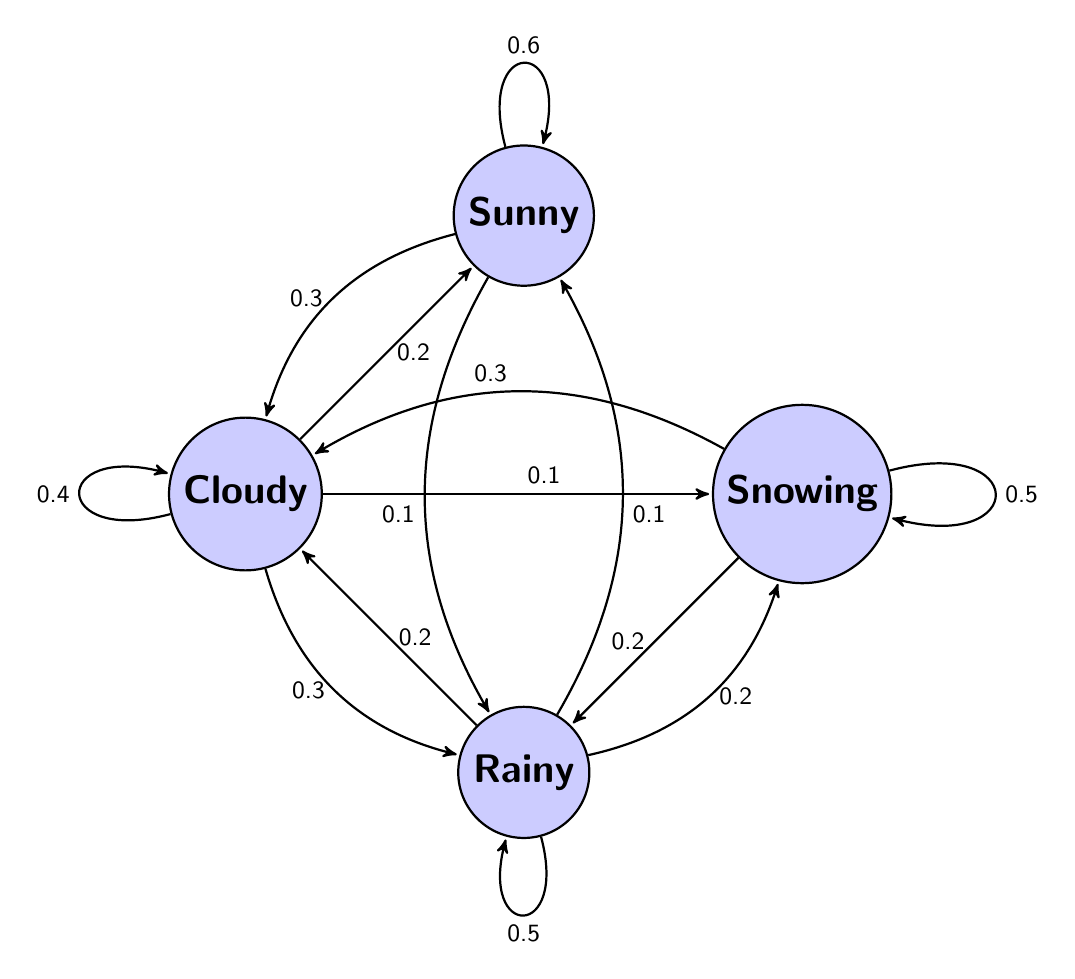
\begin{tikzpicture}[->,>=stealth',shorten >=1pt,auto,node distance=5cm,
  thick,main node/.style={circle,fill=blue!20,draw,font=\sffamily\Large\bfseries}]

  \tikzstyle{pathtaken} = [draw,line width=5pt,-,red!50]

  \node[main node] (1) {Sunny};
  \node[main node] (2) [below left of=1] {Cloudy};
  \node[main node] (3) [below right of=2] {Rainy};
  \node[main node] (4) [below right of=1] {Snowing};

  \path[every node/.style={font=\sffamily\small}]
    (1) % edge node [left] {0.0} (4) %snowing
    	edge [bend right] node [below left] {0.1} (3) %rainy
        edge [bend right] node[left] {0.3} (2) % cloudy
        edge [loop above] node {0.6} (1) % stay sunny
    (2) edge node [right] {0.2} (1)
        edge [loop left] node {0.4} (2)
        edge [bend right] node [left] {0.3} (3)
        edge node [above right] {0.1} (4)
    (3) edge [bend right] node [below right] {0.1} (1)
    	edge node [right] {0.2} (2)
    	edge [loop below] node {0.5} (3)
        edge [bend right] node[right] {0.2} (4)
    (4) edge [bend right] node [above left] {0.3} (2)
    	edge node [left] {0.2} (3)
        edge [loop right] node {0.5} (4);
\end{tikzpicture}
By simply tracing the path and multiplying up the probabilities, we can compute the
probability of a whole sequence $s_1 = $ \{cloudy, rainy, sunny, sunny\}
\begin{equation}
	p(s_1) = 1 \cdot 0.3 \cdot 0.1 \cdot 0.6 = 0.018
\end{equation}
and for the second sequence $s_2 = $ \{sunny, snowy, sunny, rainy\}
\begin{equation}
	p(s_2) = 1 \cdot 0 \cdot 0 \cdot 0.1 = 0
\end{equation}

\section*{Exercise 2}
The problem can be visualized as following graph, with each position
denoted as $\ell_i$: 
\begin{figure}[h]
\center
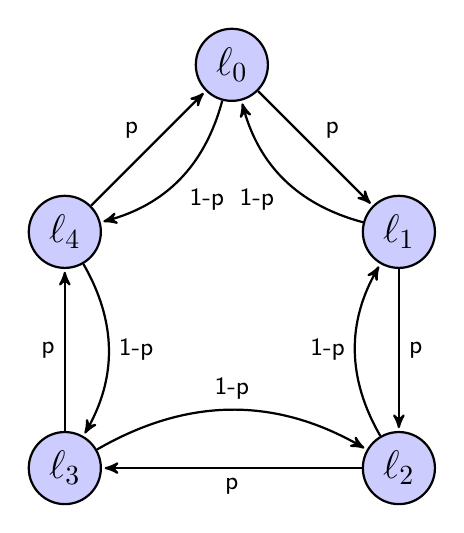
\begin{tikzpicture}[->,>=stealth',shorten >=1pt,auto,node distance=3cm,
  thick,main node/.style={circle,fill=blue!20,draw,font=\sffamily\Large\bfseries}]

  \tikzstyle{pathtaken} = [draw,line width=5pt,-,red!50]

  \node[main node] (0) {$\ell_0$};
  \node[main node] (1) [below right of=0] {$\ell_1$};
  \node[main node] (2) [below of=1] {$\ell_2$};
  \node[main node] (4) [below left of=0] {$\ell_4$};
  \node[main node] (3) [below of=4] {$\ell_3$};
  \path[every node/.style={font=\sffamily\small}]
    (0) edge node {p} (1) 
    	edge [bend left] node {1-p} (4)
    (1) edge node {p} (2) 
    	edge [bend left] node {1-p} (0)    
    (2) edge node {p} (3) 
    	edge [bend left] node {1-p} (1)
    (3) edge node {p} (4) 
    	edge [bend left] node {1-p} (2) 
    (4) edge node {p} (0) 
    	edge [bend left] node {1-p} (3);
\end{tikzpicture}
\end{figure}

\noindent
This leads to the transition matrix
\[
T_1 = 
\kbordermatrix{
    & \ell_0& \ell_1&\ell_2 & \ell_3 & \ell_4\\
\ell_0 &   0   &   p   &   0   &   0   &   1-p   \\ 
\ell_1 &   1-p   &   0   &   p   &   0   &   0   \\ 
\ell_2 &   0   &   1-p   &   0   &   p   &   0   \\ 
\ell_3 &   0   &   0   &   1-p   &   0   &   p  \\ 
\ell_4 &   p   &   0   &   0   &   1-p   &   0  \\ 
}
\]
The markov chain defined here is irreducible, since for every $l_i$ we can reach 
every other $l_j$ for every $p \in [0,1]$. If we assume $p > 0$ without loss of
generalization (just define $p' = 1 - p$ otherwise) we can simply go $4$ times into 
the direction with probability $p$ and reach every other state with a nonzero probability.

\section*{Exercise 3}
For the transition matrix
\[
T_2 = 
\kbordermatrix{
    & A& B     &  C & D     \\
A &   1   &   0   &   0   &   0   \\ 
B &   0.9   &   0   &   0.1   &   0  \\ 
C &   0   &   0.9   &   0   &   0.1   \\ 
D &   0   &   0   &   0   &   1   \\ 
}
\]
we can draw the graph as visible in Figure \ref{fig:ex3}.
\begin{figure}[h]
\center
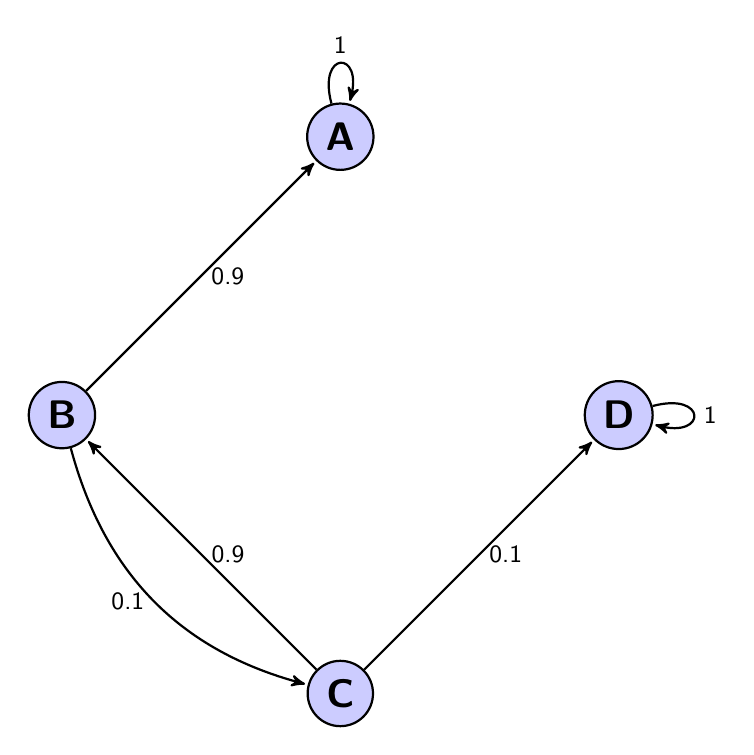
\begin{tikzpicture}[->,>=stealth',shorten >=1pt,auto,node distance=5cm,
  thick,main node/.style={circle,fill=blue!20,draw,font=\sffamily\Large\bfseries}]

  \tikzstyle{pathtaken} = [draw,line width=5pt,-,red!50]

  \node[main node] (1) {A};
  \node[main node] (2) [below left of=1] {B};
  \node[main node] (3) [below right of=2] {C};
  \node[main node] (4) [below right of=1] {D};

  \path[every node/.style={font=\sffamily\small}]
    (1) edge [loop above] node {1} (1)
    (2) edge node [right] {0.9} (1)
        
        edge [bend right] node [left] {0.1} (3)
        
    (3) 
    	edge node [right] {0.9} (2)
    	
        edge [right] node[right] {0.1} (4)
    (4) 
    
    
        edge [loop right] node {1} (4);
\end{tikzpicture}
\label{fig:ex3}
\caption{Graph of the markov chain defined for exercise 3.}
\end{figure}
First, we want to find out the probability $p_{B,A,8}$ of starting in B and ending up in A
after 8 transitions. For this we define the probability $p_l = 0.9 \cdot 0.1$ as probability of making
the loop between state B and state C. This lets us define the probability of reaching A
with infinite many transitions as
\begin{equation}
	p_{B,A,\infty} = 0.9 + p_l^1 \cdot 0.9 + p_l^2 \cdot 0.9 + p_l^3 \cdot 0.9 +  p_l^4 \cdot 0.9 + \ldots
\end{equation}
Since we are only interested in paths of lenght 8 and less, we can reduce it to the 
first four terms, since the every B-C loop takes two transitions.
\begin{align}
	p_{B,A,8} 	&= 0.9 + p_l^1 \cdot 0.9 + p_l^2 \cdot 0.9 + p_l^3 \cdot 0.9 \\
				&= 0.9889461
\end{align}
An alternative way to obtain this solution would be to compute
\begin{equation}
	\pi_B \cdot T_2^8 = [0, 1, 0, 0] \cdot T_2^8 = [0.9889, 0.0001, 0, 0.0110]
\end{equation}
Further we need to evalute the probability $p_{C,D,6}$ of being in state D after 6 
transitions when starting in state C. For this purpose we can again employ the
definition of $p_l$
\begin{equation}
	p_{C,D,\infty} = 0.1 + p_l^1 \cdot 0.1 + p_l^2 \cdot 0.1 + 
						p_l^3 \cdot 0.1 + p_l^4 \cdot 0.1 + \ldots
\end{equation}
If we again restrict ourself to 6 transitions and use the loops size of 2, we arrive at
\begin{align}
	p_{C,D,6} &= 0.1 + p_l^1 \cdot 0.1 + p_l^2 \cdot 0.1 \\
				&= 0.10981
\end{align}
Again we could use the alternative method to obtain
\begin{equation}
	\pi_C \cdot T_2^6 = [0, 0, 1, 0] \cdot T_2^6 = [ 0.8895,  0, 0.0007, 0.1098]
\end{equation}
\section*{Exercise 4}
Using the hidden markov model of the crazy machine as defined in Table \ref{tab:crazy_machine} and Figure \ref{fig:crazy_machine}, we can compute the forward probability (Table \ref{fig:crazy_forward}) and backward
probability (Table \ref{fig:crazy_backward})
probability
\begin{table}
\center
\begin{tabular}{|c|c|p{2cm}|p{3cm}|p{3.5cm}|}
	\hline
	state\textbackslash time & $t_0$ coffee 	& $t_1$ coffee & $t_2$ lemonade & $t_3$ \\  \hline
	$\alpha$(CF) 			& 1 & 0.7 * 0.6 \newline= 0.42	& 0.42 * 0.7 * 0.6 + \newline
															  0.18 * 0.5 * 0.1 \newline
															  = 0.1854 &  0.1854 * 0.7 * 0.3	+ \newline
															  			  0.0846 * 0.5 * 0.2 \newline
															  			  = 
															  	\\ \hline
	$\alpha$(WP) 			& 0 & 0.3 * 0.6 \newline = 0.18 & 0.18 * 0.5 * 0.1 + \newline
															  0.42 * 0.3 * 0.6 \newline
															  = 0.0846 &  0.1854 * 0.3 * 0.3	+ \newline
															  			  0.0846 * 0.5 * 0.2 \newline
															  			  = 		\\ \hline
	P(O) 		 			& 1 & 0.45 & 0.1854 + 0.0846 \newline 
										 = 0.27 					& 0.039519 + 0.018171 \newline
										 							  = 0.05769	\\
	\hline
\end{tabular}
\caption{The forward algorithm applied to the sequence O = \{coffee, coffee, lemonade\} }
\label{fig:crazy_forward}
\end{table}
\begin{table}
\center
\begin{tabular}{|c|p{3cm}|p{3cm}|p{3cm}|c|}
	\hline
	state\textbackslash time & $t_0$ coffee 	& $t_1$ coffee & $t_2$ lemonade & $t_3$ \\  \hline
	$\alpha$(CF) 			& 0.186 * 0.7 * 0.6 + \newline
							  0.019 * 0.5 * 0.6 \newline
							  = 0.08382 & 0.3 * 0.7 * 0.6 + \newline
								 0.2 * 0.5 * 0.6 \newline
								 = 0.186 & 0.3 & 1 \\ \hline
	$\alpha$(WP) 			& 0.186 * 0.3 * 0.1 + \newline
							  0.019 * 0.5 * 0.1 \newline
							  = 0.00653 & 0.3 * 0.3 * 0.1 + \newline
								 0.2 * 0.5 * 0.1 \newline
								 = 0.019 & 0.2 & 1		\\ \hline
	P(O) 		 			& 0.09035 & 0.205 & 	0.5	&  \\
	\hline
\end{tabular}
\caption{The backward algorithm applied to the sequence O = \{coffee, coffee, lemonade\} }
\label{fig:crazy_backward}
\end{table}
\begin{figure}[h]
\center
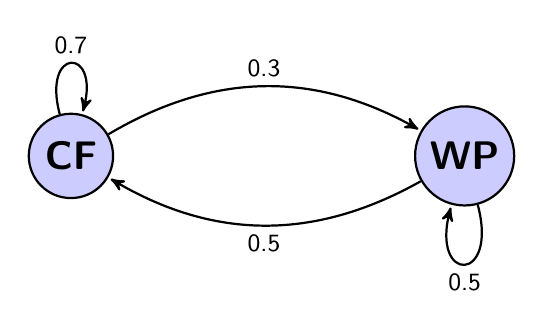
\begin{tikzpicture}[->,>=stealth',shorten >=1pt,auto,node distance=5cm,
  thick,main node/.style={circle,fill=blue!20,draw,font=\sffamily\Large\bfseries}]

  \node[main node] (1) {CF};
  \node[main node] (2) [right of=1] {WP};


  \path[every node/.style={font=\sffamily\small}]
    (1) edge [loop above] node {0.7} (1)
    	edge [bend left] node {0.3} (2)
    (2) edge [bend left] node {0.5} (1)
    	edge [loop below] node {0.5} (2);
\end{tikzpicture}
\caption{Markov chain of the crazy machine.}
\label{fig:crazy_machine}
\end{figure}
\begin{table}
\center
\begin{tabular}{|c|c|c|c|}
	\hline
	   & coffee & water & lemonade \\  \hline
	CF & 0.6 & 0.1 & 0.3 		\\ \hline
	WP & 0.1 & 0.7 & 0.2 		\\ 	
	\hline
\end{tabular}
\caption{Emission probabilities for the crazy machine.}
\label{tab:crazy_machine}
\end{table}
\end{document}